\section{Why Workflows}

%%%%%%%%%%%%%%%%%%%%%%%%%%%%%%%%%%%%%%%%%%%%%%%%%%%%%%%%%%%%%%%%%%%%%%%%%%%%%%%%
\begin{frame}
    \frametitle{Outline}
    \begin{columns}[t]
        \begin{column}{.5\textwidth}
            \tableofcontents[sections={1-9},currentsection]
        \end{column}
        \begin{column}{.5\textwidth}
            \tableofcontents[sections={10-18},currentsection]
        \end{column}
    \end{columns}
\end{frame}

%%%%%%%%%%%%%%%%%%%%%%%%%%%%%%%%%%%%%%%%%%%%%%%%%%%%%%%%%%%%%%%%%%%%%%%%%%%%%%%%
\begin{frame}
  \frametitle{What is this about?}
   \question[Questions]{\begin{itemize}
                         \item I can code everything! Can I?
                         \item What is the benefit of a workflow system?
                         \item What distinguishes a workflow system from a ``pipeline''?
                        \end{itemize}
                       }
   \docs[Objectives]{\begin{enumerate}
                      \item Introducing workflow engines (particularly \texttt{Snakemake})!
                     \end{enumerate}}
\end{frame}  

%%%%%%%%%%%%%%%%%%%%%%%%%%%%%%%%%%%%%%%%%%%%%%%%%%%%%%%%%%%%%%%%%%%%%%%%%%%%%%%%
\begin{frame}
  \frametitle{Data Analysis}
  \begin{onlyenv}<1| handout:0>
    \begin{tikzpicture}
      \path[use as bounding box] (0.7,0) rectangle (12,8);
      \node[inner sep=0pt] (analysis_1) at (5,6)
         {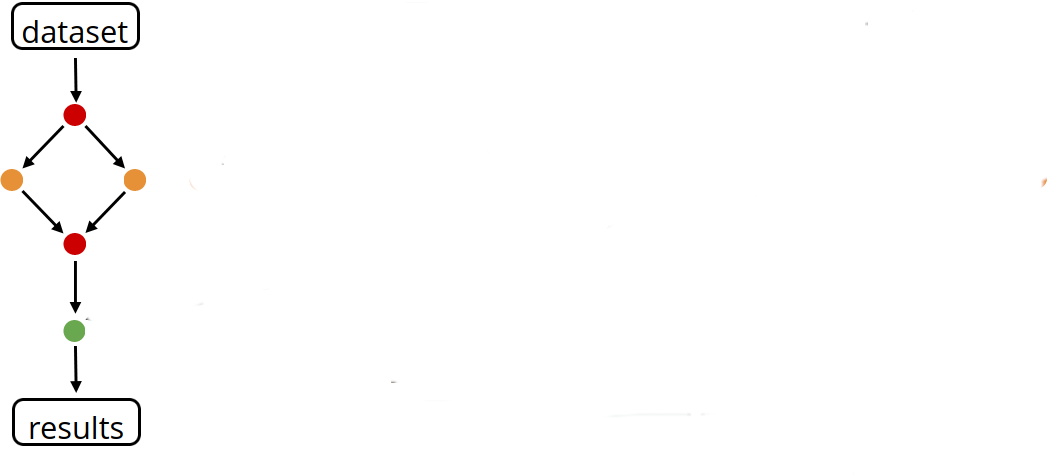
\includegraphics[width=0.7\textwidth]{Snakemake/analysis_1.png}};   
      \node at (7, 3.5) %[below=-0.4cm of analysis_1, xshift=2.7cm] at (current page.center)
         {
\includegraphics[width=0.45\textwidth]{Snakemake/phd_left.png}};
      \node at (6, 1) {\begin{minipage}{0.75\textwidth}\footnotesize
                        Idea from the official \lhref{https://slides.com/johanneskoester/snakemake-tutorial}{\texttt{Snakemake}} course (with permission), image from \lhref{https://phdcomics.com/comics.php}{PhD comics}.
                       \end{minipage}
      };
    \end{tikzpicture}    
  \end{onlyenv}
  
  \begin{onlyenv}<2| handout:1>
    \begin{tikzpicture}
      \path[use as bounding box] (0.7,0) rectangle (12,8);
      \node[inner sep=0pt] (analysis_full) at (5,6)
         {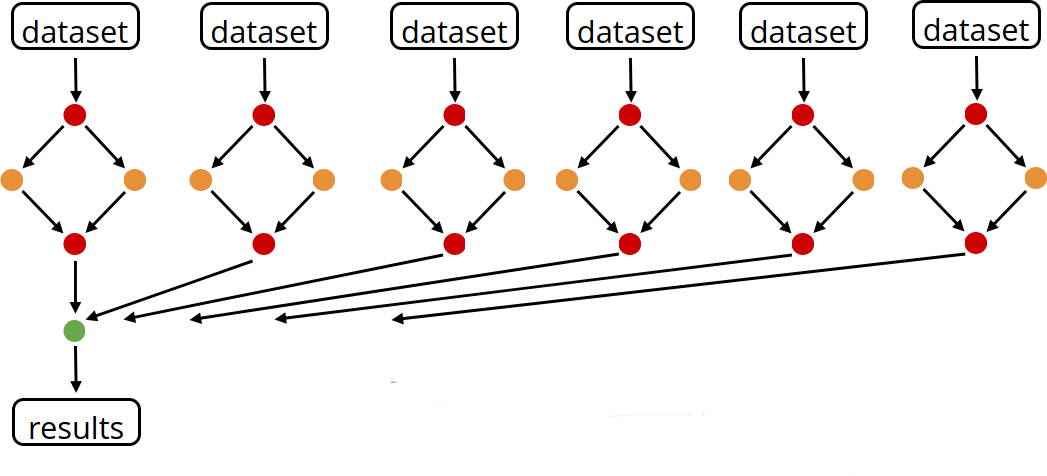
\includegraphics[width=0.7\textwidth]{Snakemake/analysis_full.png}};   
      \node at (7,3.5) % [below=-0.4cm of analysis_full, xshift=2.7cm]
         {
\includegraphics[width=0.45\textwidth]{Snakemake/phd_full.png}};
      \node at (6, 1) {\begin{minipage}{0.75\textwidth}\footnotesize
                        Idea from the official \lhref{https://slides.com/johanneskoester/snakemake-tutorial}{\texttt{Snakemake}} course (with permission), image from \lhref{https://phdcomics.com/comics.php}{PhD comics}.
                       \end{minipage}
      };
    \end{tikzpicture}
  \end{onlyenv}
\end{frame}

%%%%%%%%%%%%%%%%%%%%%%%%%%%%%%%%%%%%%%%%%%%%%%%%%%%%%%%%%%%%%%%%%%%%%%%%%%%%%%%%
\begin{frame}
  \frametitle{Reproducible Data Analysis}
  \begin{onlyenv}<1| handout:0>
    \begin{tikzpicture}
      \path[use as bounding box] (0.7,0) rectangle (12,8);
      \node at (5.5, 5.5) {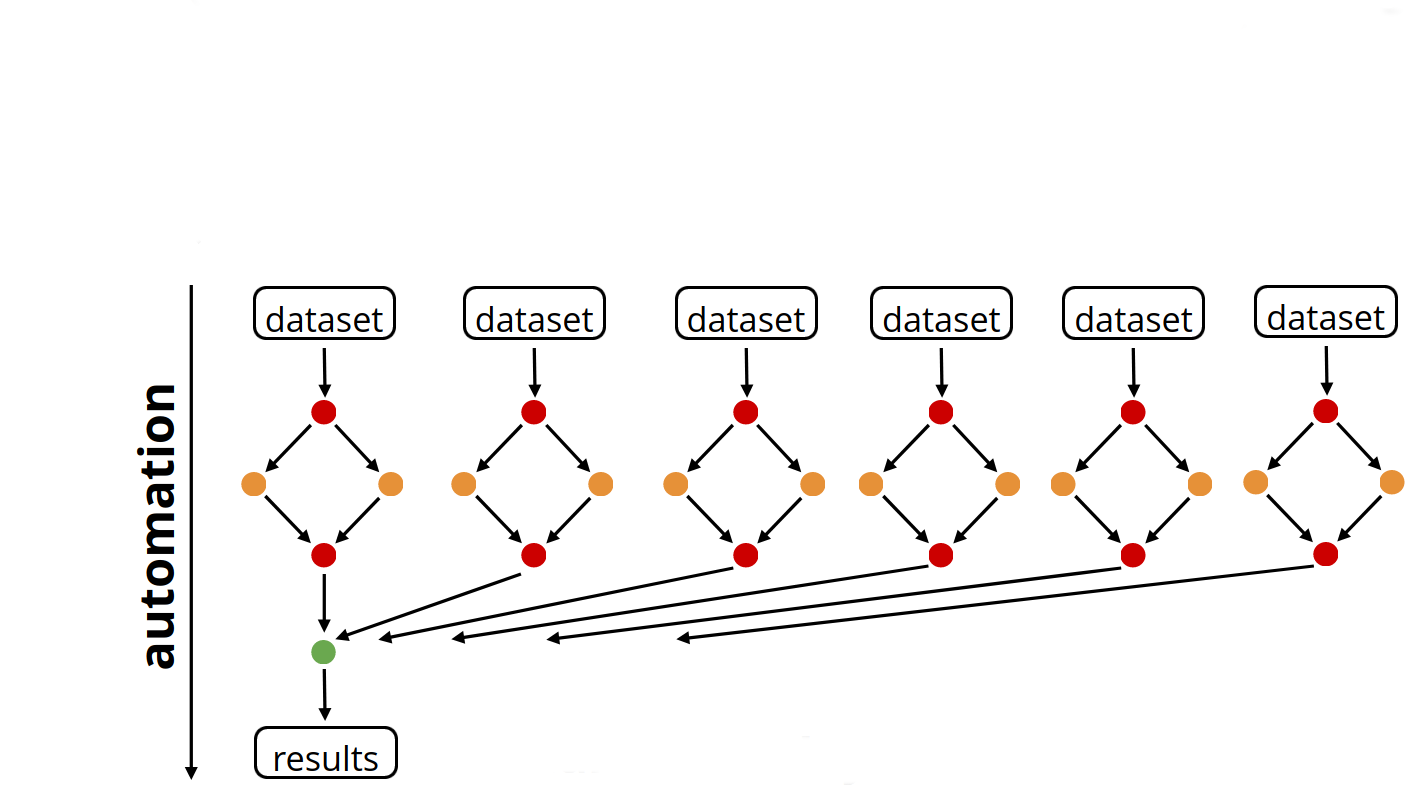
\includegraphics[width=0.7\textwidth]{Snakemake/automation.png}};
      \node at (8, 2.5) {\begin{minipage}{0.65\textwidth}
                             \textbf{From raw data to final figures:}
                             \begin{itemize}
                                \item \textbf{document} parameters, tools, versions
                                \item \textbf{execute} without manual intervention
                              \end{itemize}
                           \end{minipage}
                           };
    \end{tikzpicture}
  \end{onlyenv}
  \begin{onlyenv}<2| handout:0>
    \begin{tikzpicture}
      \path[use as bounding box] (0.7,0) rectangle (12,8);
      \node at (5.5, 5.5) {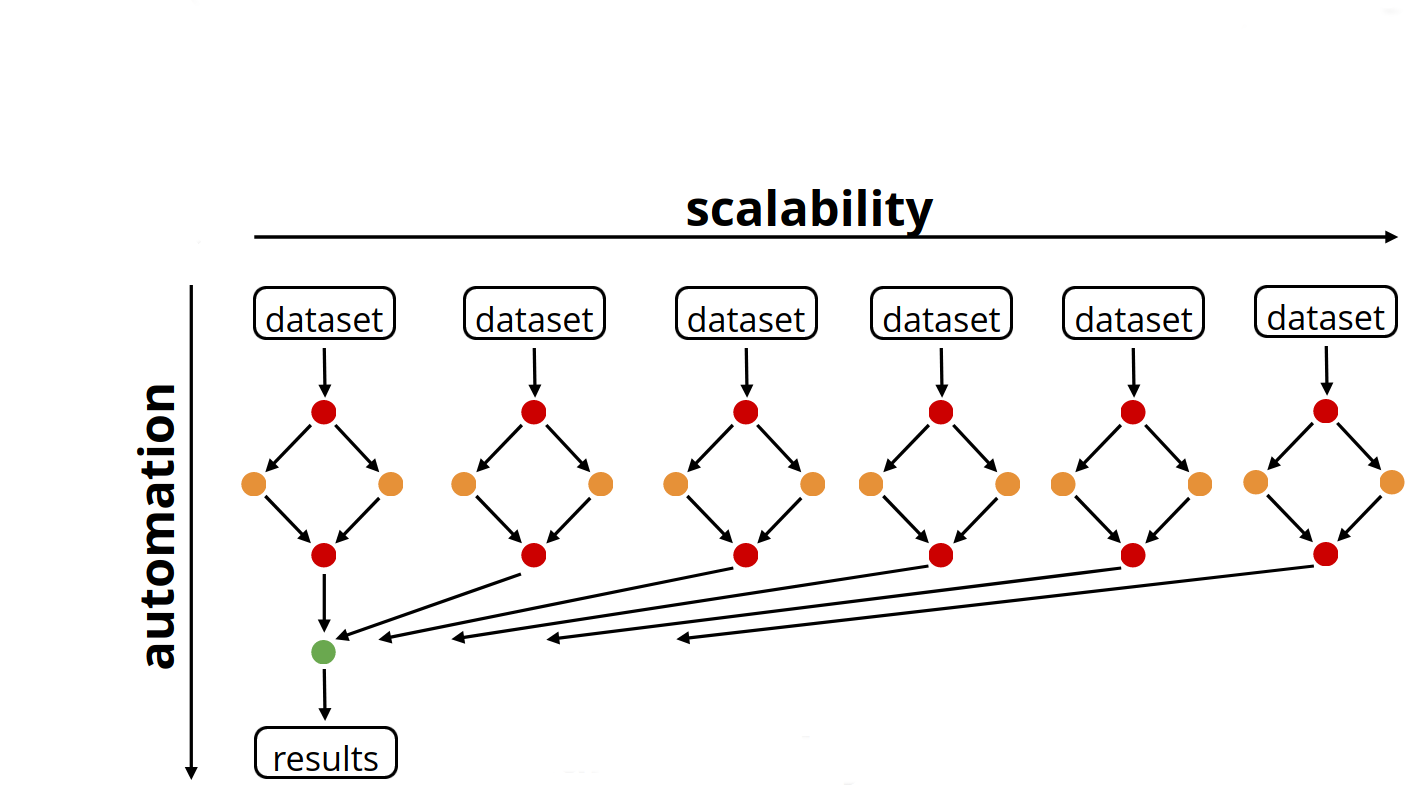
\includegraphics[width=0.7\textwidth]{Snakemake/scalability.png}};
      \node at (8, 2.5) {\begin{minipage}{0.65\textwidth}
                             \textbf{Handle parallelization:}
                             \begin{itemize}
                                \item execute for tens of thousands of datasets
                                \item efficiently use any computing platform
                              \end{itemize}
                           \end{minipage}
                           };
    \end{tikzpicture}
  \end{onlyenv}
  \begin{onlyenv}<3| handout:1>
    \begin{tikzpicture}
      \path[use as bounding box] (0.7,0) rectangle (12,8);
      \node at (5.5, 5.5) {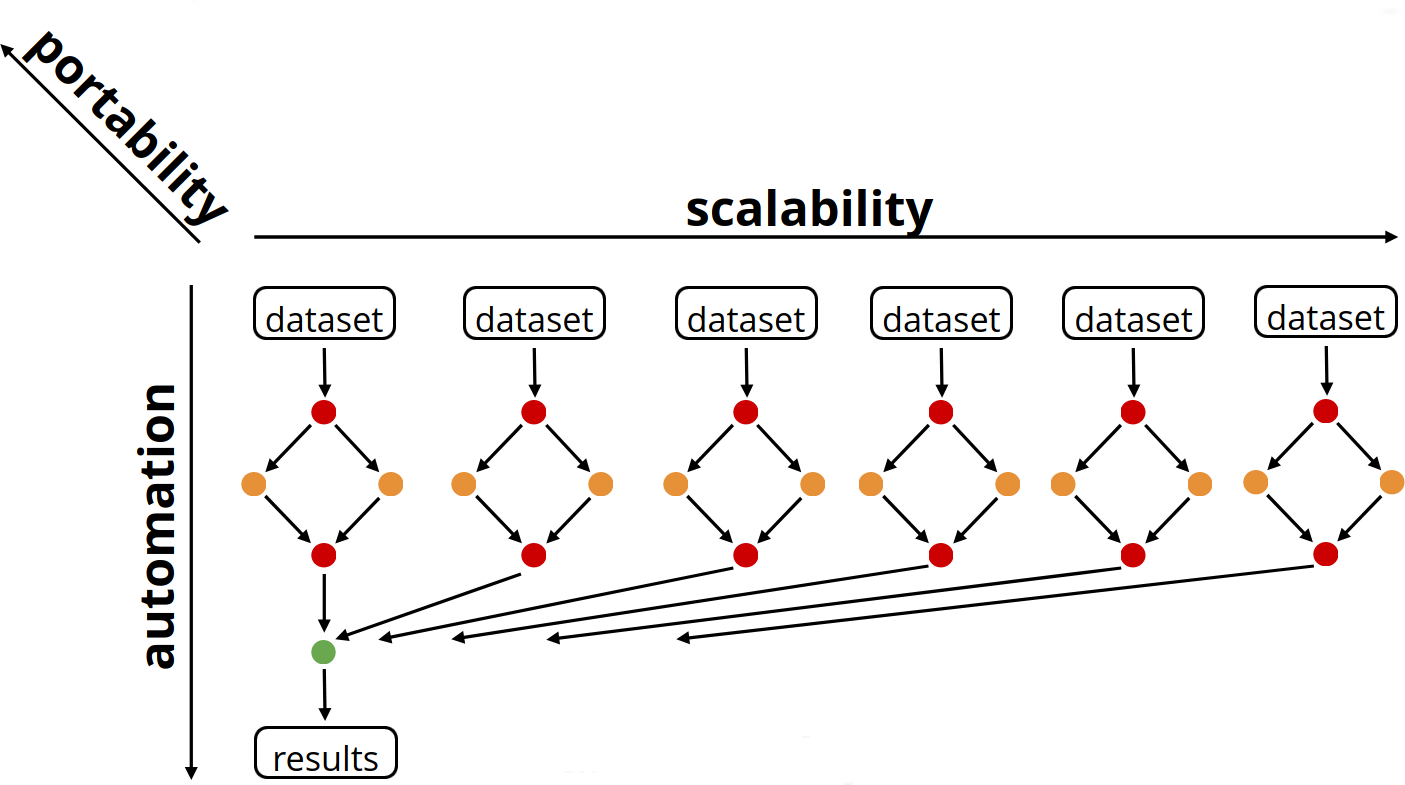
\includegraphics[width=0.7\textwidth]{Snakemake/portability.png}};
      \node at (8, 2.5) {\begin{minipage}{0.65\textwidth}
                             \textbf{Handle deployment:}\newline
                             be able to easily execute analyses on a different system/platform/infrastructure
                           \end{minipage}
                           };
    \end{tikzpicture}
  \end{onlyenv}
\end{frame}

%%%%%%%%%%%%%%%%%%%%%%%%%%%%%%%%%%%%%%%%%%%%%%%%%%%%%%%%%%%%%%%%%%%%%%%%%%%%%%%%
\begin{frame}
  \frametitle{Beyond Reproducibility}
  \begin{onlyenv}<1| handout:0>
    \begin{figure}
      \centering
      
\includegraphics[width=0.85\textwidth]{Snakemake/reproducibility_only.png}
    \end{figure}
  \end{onlyenv}
  \begin{onlyenv}<2| handout:0>
    \begin{figure}
      \centering
      
\includegraphics[width=0.85\textwidth]{Snakemake/reproducibility_empty.png}
    \end{figure}
  \end{onlyenv}
  \begin{onlyenv}<3| handout:0>
    \begin{figure}
      \centering
      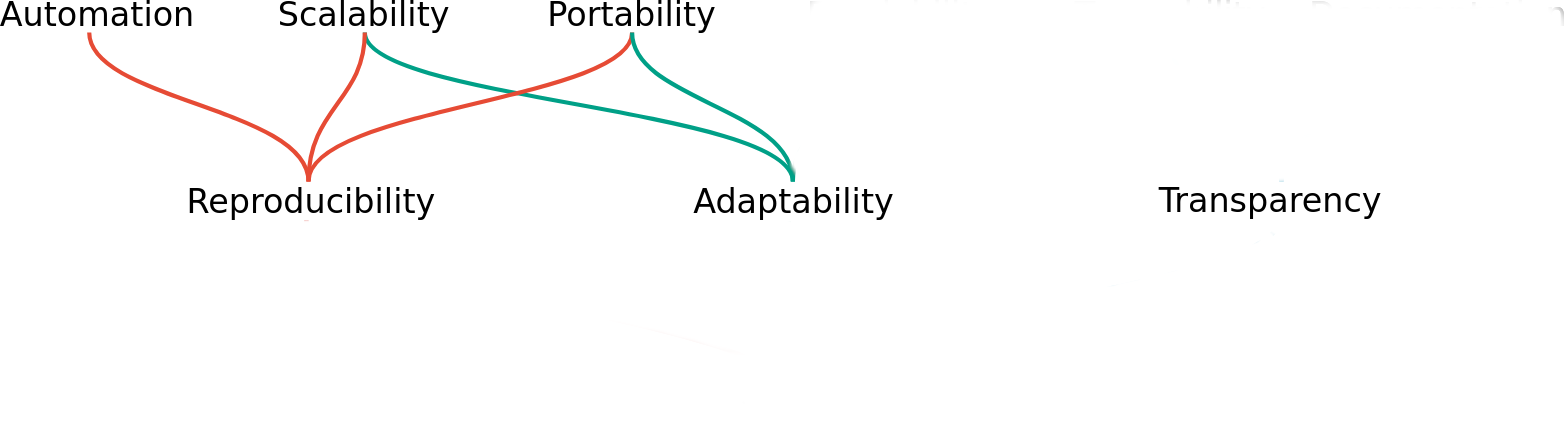
\includegraphics[width=0.85\textwidth]{Snakemake/reproducibility_left.png}
    \end{figure}
  \end{onlyenv}
    \begin{onlyenv}<4| handout:1>
      \begin{figure}
        \centering
        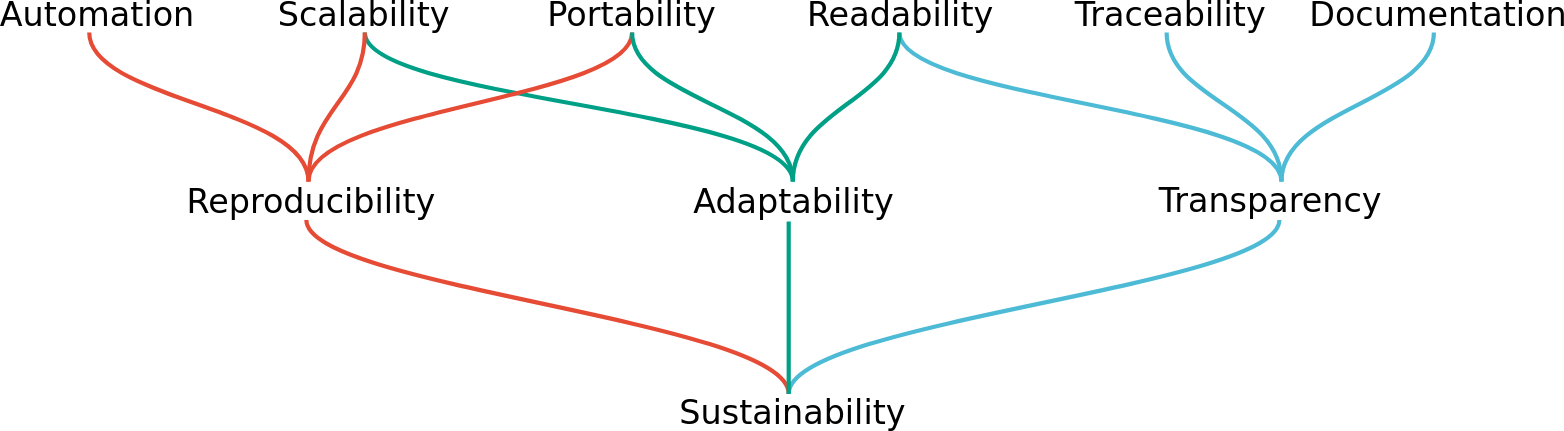
\includegraphics[width=0.85\textwidth]{Snakemake/reproducibility_full.png}
      \end{figure}
  \end{onlyenv}
\end{frame}
